\documentclass{article}

\usepackage[utf8]{inputenc}
\usepackage[frenchb]{babel}
\usepackage[T1]{fontenc}
\usepackage{graphicx}
\usepackage{amsmath,amsfonts,amssymb}
\usepackage{pgfplots}
\usepackage{lscape}
\usepackage{braket}
\usepackage{multirow}
\usepackage{hyperref}
\usepackage{listings}
\usepackage{color}
\usepackage{float}
\usepackage{ulem}
\usepackage{framed}
\definecolor{lightgray}{rgb}{.9,.9,.9}
\definecolor{darkgray}{rgb}{.4,.4,.4}
\definecolor{purple}{rgb}{0.65, 0.12, 0.82}

\newcommand{\Sha}{\textls[0]{III}}

\lstdefinelanguage{JavaScript}{
  keywords={include, mesh, physical, group, function, jacobian, integration, constraint, functionspace, formulation, resolution, postprocessing, postoperation, name, case, operation},
  keywordstyle=\color{blue}\bfseries,
  ndkeywords={class, export, boolean, throw, implements, import, this},
  ndkeywordstyle=\color{darkgray}\bfseries,
  identifierstyle=\color{black},
  sensitive=false,
  comment=[l]{//},
  morecomment=[s]{/*}{*/},
  commentstyle=\color{purple}\ttfamily,
  stringstyle=\color{red}\ttfamily,
  morestring=[b]',
  morestring=[b]"
}

\lstset{
   language=JavaScript,
   extendedchars=true,
   basicstyle=\footnotesize\ttfamily,
   showstringspaces=false,
   showspaces=false,
   numbers=left,
   numberstyle=\footnotesize,
   numbersep=9pt,
   tabsize=2,
   breaklines=true,
   showtabs=false,
   captionpos=b
}

\usepackage[europeanvoltages, europeancurrents, europeanresistors, americaninductors]{circuitikz}

\usepackage{fancyhdr}
\usepackage[headheight = 2cm,bottom=3.5cm]{geometry}
\pagestyle{fancy}
\renewcommand{\headrulewidth}{1pt}
\fancyhead[L]{\includegraphics[height=1.5cm]{assets/logocs.png}} 
\fancyhead[C]{\textsc{Performance analysis of a batched\\ parallel reduction using CUDA\\}}
\fancyhead[R]{\includegraphics[height=1.5cm]{assets/soprasteria.png}}
\renewcommand{\footrulewidth}{1pt}
\fancyfoot[C]{} 
\fancyfoot[L]{\href{https://drive.google.com/open?id=1ETwTI8ptyoaDpvvjFe6wB5ziKXfQL0BL}{Baptiste Legouix}}


\begin{document}
\title{\vspace{-70pt}\textsc{CS Group} \\
\vspace{10pt}\hspace*{-25pt}\begin{tabular}{cc}
\multirow{4}{*}{
\begin{minipage}{0.20\textwidth}\vspace{15pt}\includegraphics[scale=0.53]{assets/biglogocs.png}\end{minipage}} & \rule{0.60\linewidth}{0.5pt}\vspace{10pt} \\ & Performance analysis of a batched\\ & parallel reduction using CUDA\\ & \rule{0.60\linewidth}{2pt}
\end{tabular}}
\author{\href{https://drive.google.com/open?id=1ETwTI8ptyoaDpvvjFe6wB5ziKXfQL0BL}{Baptiste Legouix}}
%\date{\today\\[30pt] \huge \ccbynd}
\date{\today}

\clearpage
\maketitle
\thispagestyle{empty}

\vspace{0pt}
\begin{center}
\includegraphics[width=0.7\textwidth]{assets/cover.png}
\end{center}
\vspace{0pt}

\tableofcontents

\vspace{30pt}

\subsection*{Abstract}

placeholder

\newpage

\setcounter{page}{1}
\fancyfoot[R]{\thepage}

\section{Presentation}

% \subsection*{Introduction}

\subsection{GPU Architecture}

\textit{Graphical Processor Units} differentiate themselves from CPU by relying on the SIMT (Single-Instruction, Multiple Threads) execution model. It means an instruction in a CUDA computing kernel has to be executed by all the \textit{threads} forming a \textit{warp}, synchronously.

The hardware architecture of the GPU is as follow:

\begin{figure}[H]
\begin{center}
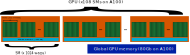
\includegraphics[width=\textwidth]{assets/gpu_arch.png}
\end{center}
\label{fig:gpu_arch}
\end{figure}

If threads inside a warp are automatically synchronized due to the SIMT model (an instruction has to be executed by all the threads within the warp before executing the next one), warps within a \textit{Stream Multiprocessor} or SMs within the GPU are running concurrently but not synchronously. It means warps and SM have to be synchronized using dedicated CUDA instruction to prevent race conditions.

Note: if threads within a warp are running synchronously, the \textit{ordering} of the execution is undetermined (we do not know which thread will be the first to finish the execution of a single instruction).

Note: since CUDA 9 the SIMT model has been slightly relaxed which can lead to subtle desynchronizations within a warp, which justify the need for the \textit{\_\_syncwarp()} CUDA function.

\subsection{CUDA programming model}

CUDA is the native language provided by Nvidia (chip manufacturer) to program for GPU. It relies on \textit{CUDA kernels} which contain the code to be executed on the GPU. 

The calls of launching CUDA kernels are parametrized with two compile-time integers: the \textit{grid size} and the \emph{block size}. Those two numbers correspond respectively to the number of SM and the number of threads per SM to be used by the CUDA kernel. If the block size is not a multiple of the warp size (32 in every current architectures), the compiler will automatically mask off exceding threads.

placeholder\cite{cudasharedmemory}

\newpage
\nocite{*}
\bibliographystyle{unsrt}
\bibliography{biblio}

\end{document}
